%%%%%%%%%%%%%%%%%%%%%%%%%%%%%%%%%%%%%%%%%
% UH Manoa ECE Capstone Poster
% Transformer-Based Lossless Source Coding
% Dan Vu, Yixin Zhang, Spring 2026
% Advisor: Prof. Anders Host-Madsen
%%%%%%%%%%%%%%%%%%%%%%%%%%%%%%%%%%%%%%%%%

\documentclass[final]{beamer}

\usepackage[scale=1.15]{beamerposter}

%----------------------------------------------------------
% UH Manoa color palette
%----------------------------------------------------------
\definecolor{uhgreen}{RGB}{0,112,48}
\definecolor{uhgreenlight}{RGB}{232,245,238}
\definecolor{alertred}{RGB}{174,32,18}
\definecolor{tealblue}{RGB}{0,95,115}

\setbeamercolor{block title}{fg=uhgreen,bg=white}
\setbeamercolor{block body}{fg=black,bg=white}
\setbeamercolor{block alerted title}{fg=white,bg=uhgreen}
\setbeamercolor{block alerted body}{fg=black,bg=uhgreenlight}

%----------------------------------------------------------
% Layout
%----------------------------------------------------------
\newlength{\sepwid}
\newlength{\leftcolwid}
\newlength{\rightcolwid}
\setlength{\paperwidth}{48in}
\setlength{\paperheight}{36in}
\setlength{\sepwid}{0.015\paperwidth}
\setlength{\leftcolwid}{0.520\paperwidth}
\setlength{\rightcolwid}{0.400\paperwidth}
\setlength{\topmargin}{-0.7in}

%----------------------------------------------------------
\usepackage{graphicx}
\usepackage{booktabs}
\usepackage{amsmath,amssymb}
\usepackage{array}
\usepackage{xcolor}
\usepackage{caption}
\usepackage{multirow}

%----------------------------------------------------------
\title{\textbf{Learned Lossless Source Coding}}
\author{Dan Vu \and Yixin Zhang \and Advisor: Prof.\ Anders H\o{}st-Madsen}
\institute{Department of Electrical \& Computer Engineering,
           University of Hawai\textquoteleft{}i at M\=anoa}

%----------------------------------------------------------
\begin{document}

\addtobeamertemplate{block end}{}{\vspace*{1.5ex}}
\addtobeamertemplate{block alerted end}{}{\vspace*{1.5ex}}
\setlength{\belowcaptionskip}{1ex}
\setlength\belowdisplayshortskip{1ex}

\begin{frame}[t]

%==========================================================
%  HEADER
%==========================================================
\begin{columns}[t]
  \begin{column}{0.15\paperwidth}
    \vspace{0.5ex}\hspace{0.5em}
    
\includegraphics[width=0.85\linewidth]{figures/uh_logo.png}
  \end{column}
  \begin{column}{0.70\paperwidth}
    \centering
    {\Huge\textbf{Transformer Based Lossless Source Coding}}\\[0.9ex]
    {\Large\textbf{Benchmarking Classical and Learned Compressors}}\\[0.5ex]
    {\large Dan Vu \quad Yixin Zhang \quad Advisor: Prof.\ Anders H\o{}st-Madsen }\\[0.3ex]
    {\normalsize Department of Electrical \& Computer Engineering,
     University of Hawai\textquoteleft{}i at M\=anoa}
  \end{column}
  \begin{column}{0.15\paperwidth}
    \vspace{0.5ex}\hspace{0.8em}
    
\includegraphics[width=0.85\linewidth]{figures/ece_logo.png}
  \end{column}
\end{columns}

\vspace{1ex}
\rule{\linewidth}{2pt}
\vspace{1ex}

%=========================================================
%  BODY
%==========================================================
\begin{columns}[t]

\begin{column}{\sepwid}\end{column}

%==========================================================
%  LEFT COLUMN
%==========================================================
\begin{column}{\leftcolwid}

%----------------------------------------------------------
\begin{block}{Introduction \& Motivation}

\textbf{Why lossless compression?}
Digital data transmission and storage demand efficient encoding with zero information loss.
Lossless compression is critical in applications ranging from file archiving and 
streaming media to DNA sequencing and network packet transmission.
The theoretical lower bound on average code length is the \textbf{Shannon entropy} $H$ (bits/symbol).

\medskip
\textbf{Entropy of a binary source:}
For a Bernoulli($p$) source, the binary entropy is
\[
  H(p) = -p\log_2 p - (1-p)\log_2(1-p).
\]
and no lossless coder can achieve average bits per symbol below $H(p)$.

\medskip
\textbf{How does arithmetic coding work?}
We evaluate each compressor by the bits-per-symbol (BPS) it achieves under arithmetic coding, where the codelength is determined by the model's sequential predictions $\hat{P}(x_n \mid x_1, \ldots, x_{n-1})$. A compressor achieves $\text{BPS} \approx H$ if and only if its probability model is accurate.
\[
  \text{BPS} = \frac{1}{N}\sum_{n=1}^{N} -\log_2 \hat{P}(x_n \mid x_{<n}).
\]
Better probability estimates $\Rightarrow$ lower BPS $\Rightarrow$ better compression.

\medskip

\textbf{Learned estimator and redundancy:}
The redundancy of a learned coder is defined as
\[
    R_l(L, m, \theta) = \frac{1}{l} E_\theta[L(x^l; x^m)] - H_\theta(X)
\]
where the expectation is taken over test sequences $x^l$ given fixed training data $x^m$, 
and $H_\theta(X)$ is the true entropy rate of the source. Redundancy measures the 
excess codelength beyond the theoretical minimum.


\medskip
\textbf{Classical compression baselines:}
\begin{itemize}
  \item \textbf{Laplace estimation:} $\hat{p} = (k+1)/(n+2)$; optimal for i.i.d.\ sources; assumes no temporal structure.
  \item \textbf{Context Tree Weighting (CTW):} tree-based sequential estimator; requires warmup. Source code: gabescahmberg, Github 
\end{itemize}

\medskip
\textbf{The theoretical question} (H\o{}st-Madsen 2020): how much training data $m$ is needed
to beat a universal source coder? Theory predicts $m \propto \ell/\!\log\ell$, a surprisingly small requirement.
\textbf{We test this empirically} using a frozen transformer as the learned estimator.

\medskip
\textbf{Our hypothesis:} A pre-trained transformer can learn arbitrary sequential
dependencies, matching or beating classical methods with only moderate training.

\end{block}

%----------------------------------------------------------
\begin{block}{Architecture \& Methods}

\begin{columns}[t]
  \begin{column}{0.46\linewidth}
    \textbf{Transformer (minGPT-nano):}
    \begin{itemize}
      \item 0.11M parameters
      \item Block size: 499 tokens
      \item Vocabulary: binary $\{0,1\}$
      \item Trained offline; \textbf{frozen} at test time
    \end{itemize}

    \medskip
    \textbf{Training:} next-bit cross-entropy loss,
    500--1000 iterations on 10{,}000 pre-generated
    sequences of length 500.
  \end{column}
  \begin{column}{0.50\linewidth}
    \textbf{Evaluation protocol:}
    \begin{itemize}
      \item Three source types: IID Bernoulli, 4-state FSM
      \item Sequence lengths $N \in \{10,25,50,100,200,300,499\}$
      \item 100 independent test sequences per condition
      \item \textbf{Redundancy} $= \text{BPS} - H(\text{source})$;\\
            a perfect coder achieves redundancy $= 0$
    \end{itemize}

    \medskip
    \textbf{CTW:} depth$=8$; KT estimators; beta-weighted
    mixing (gabeschamberg implementation).
  \end{column}
\end{columns}

\end{block}

%----------------------------------------------------------
\begin{block}{IID Sources: Baseline Behavior}

On IID Bernoulli sources, the transformer has \textbf{no exploitable structure} to
learn. As expected, it performs on par with Laplace estimation across all $p$ values and
sequence lengths with both converging to the entropy floor $H(p)$.

\begin{center}
  
\includegraphics[width=\linewidth]{figures/iid_bps_per_p.png}
\end{center}
{\small \textbf{Figure 1.} BPS vs.\ sequence length $N$ for IID Bernoulli sources at five
bias values. Transformer ({\color{tealblue}$\blacksquare$}) and Laplace
({\color{alertred}$\bullet$}) track each other closely at all $N$; both approach the
entropy floor (dotted line). Error bars show $\pm 1$ standard error over 100 trials.
This establishes the baseline: for structureless sources, learned and classical methods
are equivalent.}

\end{block}

%----------------------------------------------------------
\begin{block}{Conclusion}

\begin{itemize}
  \item \textbf{IID sources:} Transformer $\approx$ Laplace; no exploitable structure; training redundancy decays at $O(1/m)$ rate. Specialized training grants an immediate advantage at small $N$.
  \item \textbf{FSM sources:} Transformer beats both Laplace \emph{and} CTW at every $N$ tested, small $N$ is where CTW's warmup cost is prohibitive.
  \item \textbf{Learning rate:} Redundancy crosses Laplace near $m \approx 80$,
        confirming $m \propto \ell/\!\log\ell$ empirically.
  \item \textbf{Future work:} Larger alphabets, longer sequences, larger models, advanced Markov models 
\end{itemize}

\end{block}

%----------------------------------------------------------
\end{column} % end LEFT COLUMN

\begin{column}{\sepwid}\end{column}

%==========================================================
%  RIGHT COLUMN
%==========================================================
\begin{column}{\rightcolwid}

%----------------------------------------------------------
\begin{block}{Results \& Analysis}

%----- Specialized IID --------------------------------
\textbf{Transformer models trained on a specific source beat Laplace immediately.}
When the transformer is trained on a \emph{specific} $p$ value, it encodes that prior
knowledge into its weights. At test time it does not need to estimate $p$ from scratch
since it already knows the distribution.

\begin{columns}[t]
  \begin{column}{0.4\linewidth}
    \begin{center}
      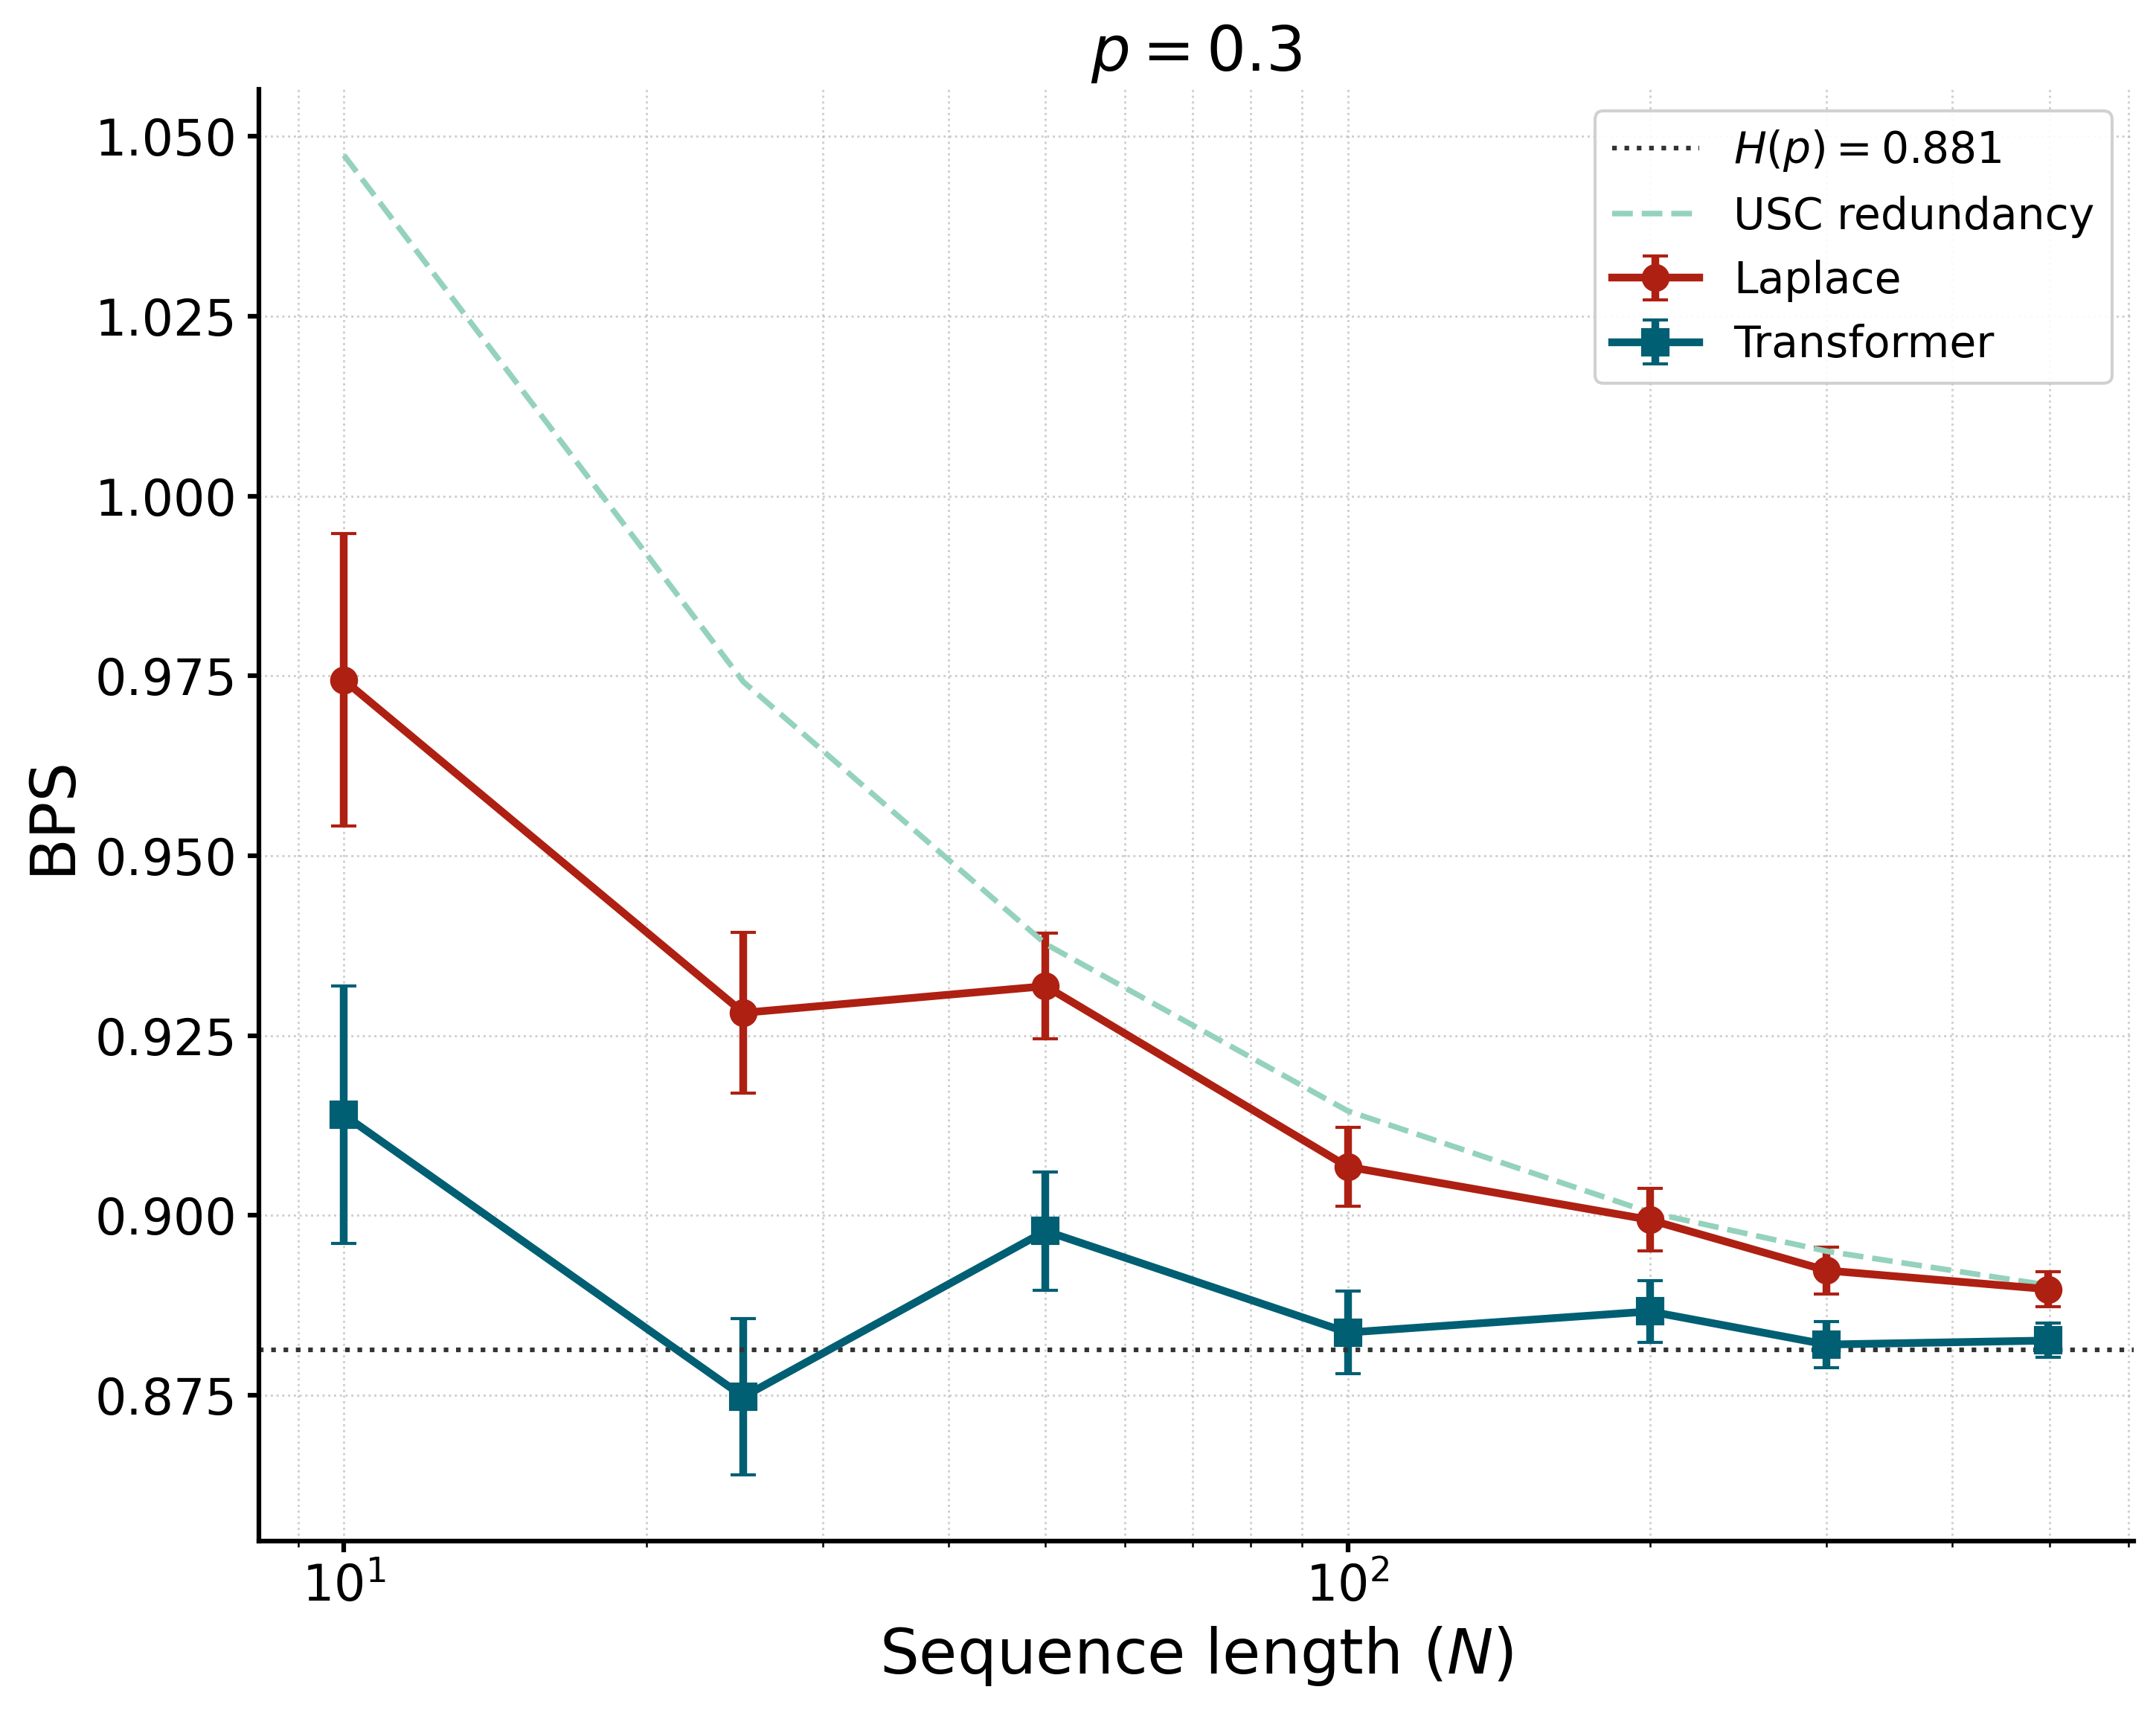
\includegraphics[width=\linewidth]{figures/iid_bps_p03.png}
    \end{center}
    {\small \textbf{Figure 2a.} Specialized model ($p{=}0.3$). Transformer beats Laplace
    at \emph{every} $N$, including $N{=}10$ where Laplace has seen almost no data.}
  \end{column}
  \begin{column}{0.4\linewidth}
    \begin{center}
      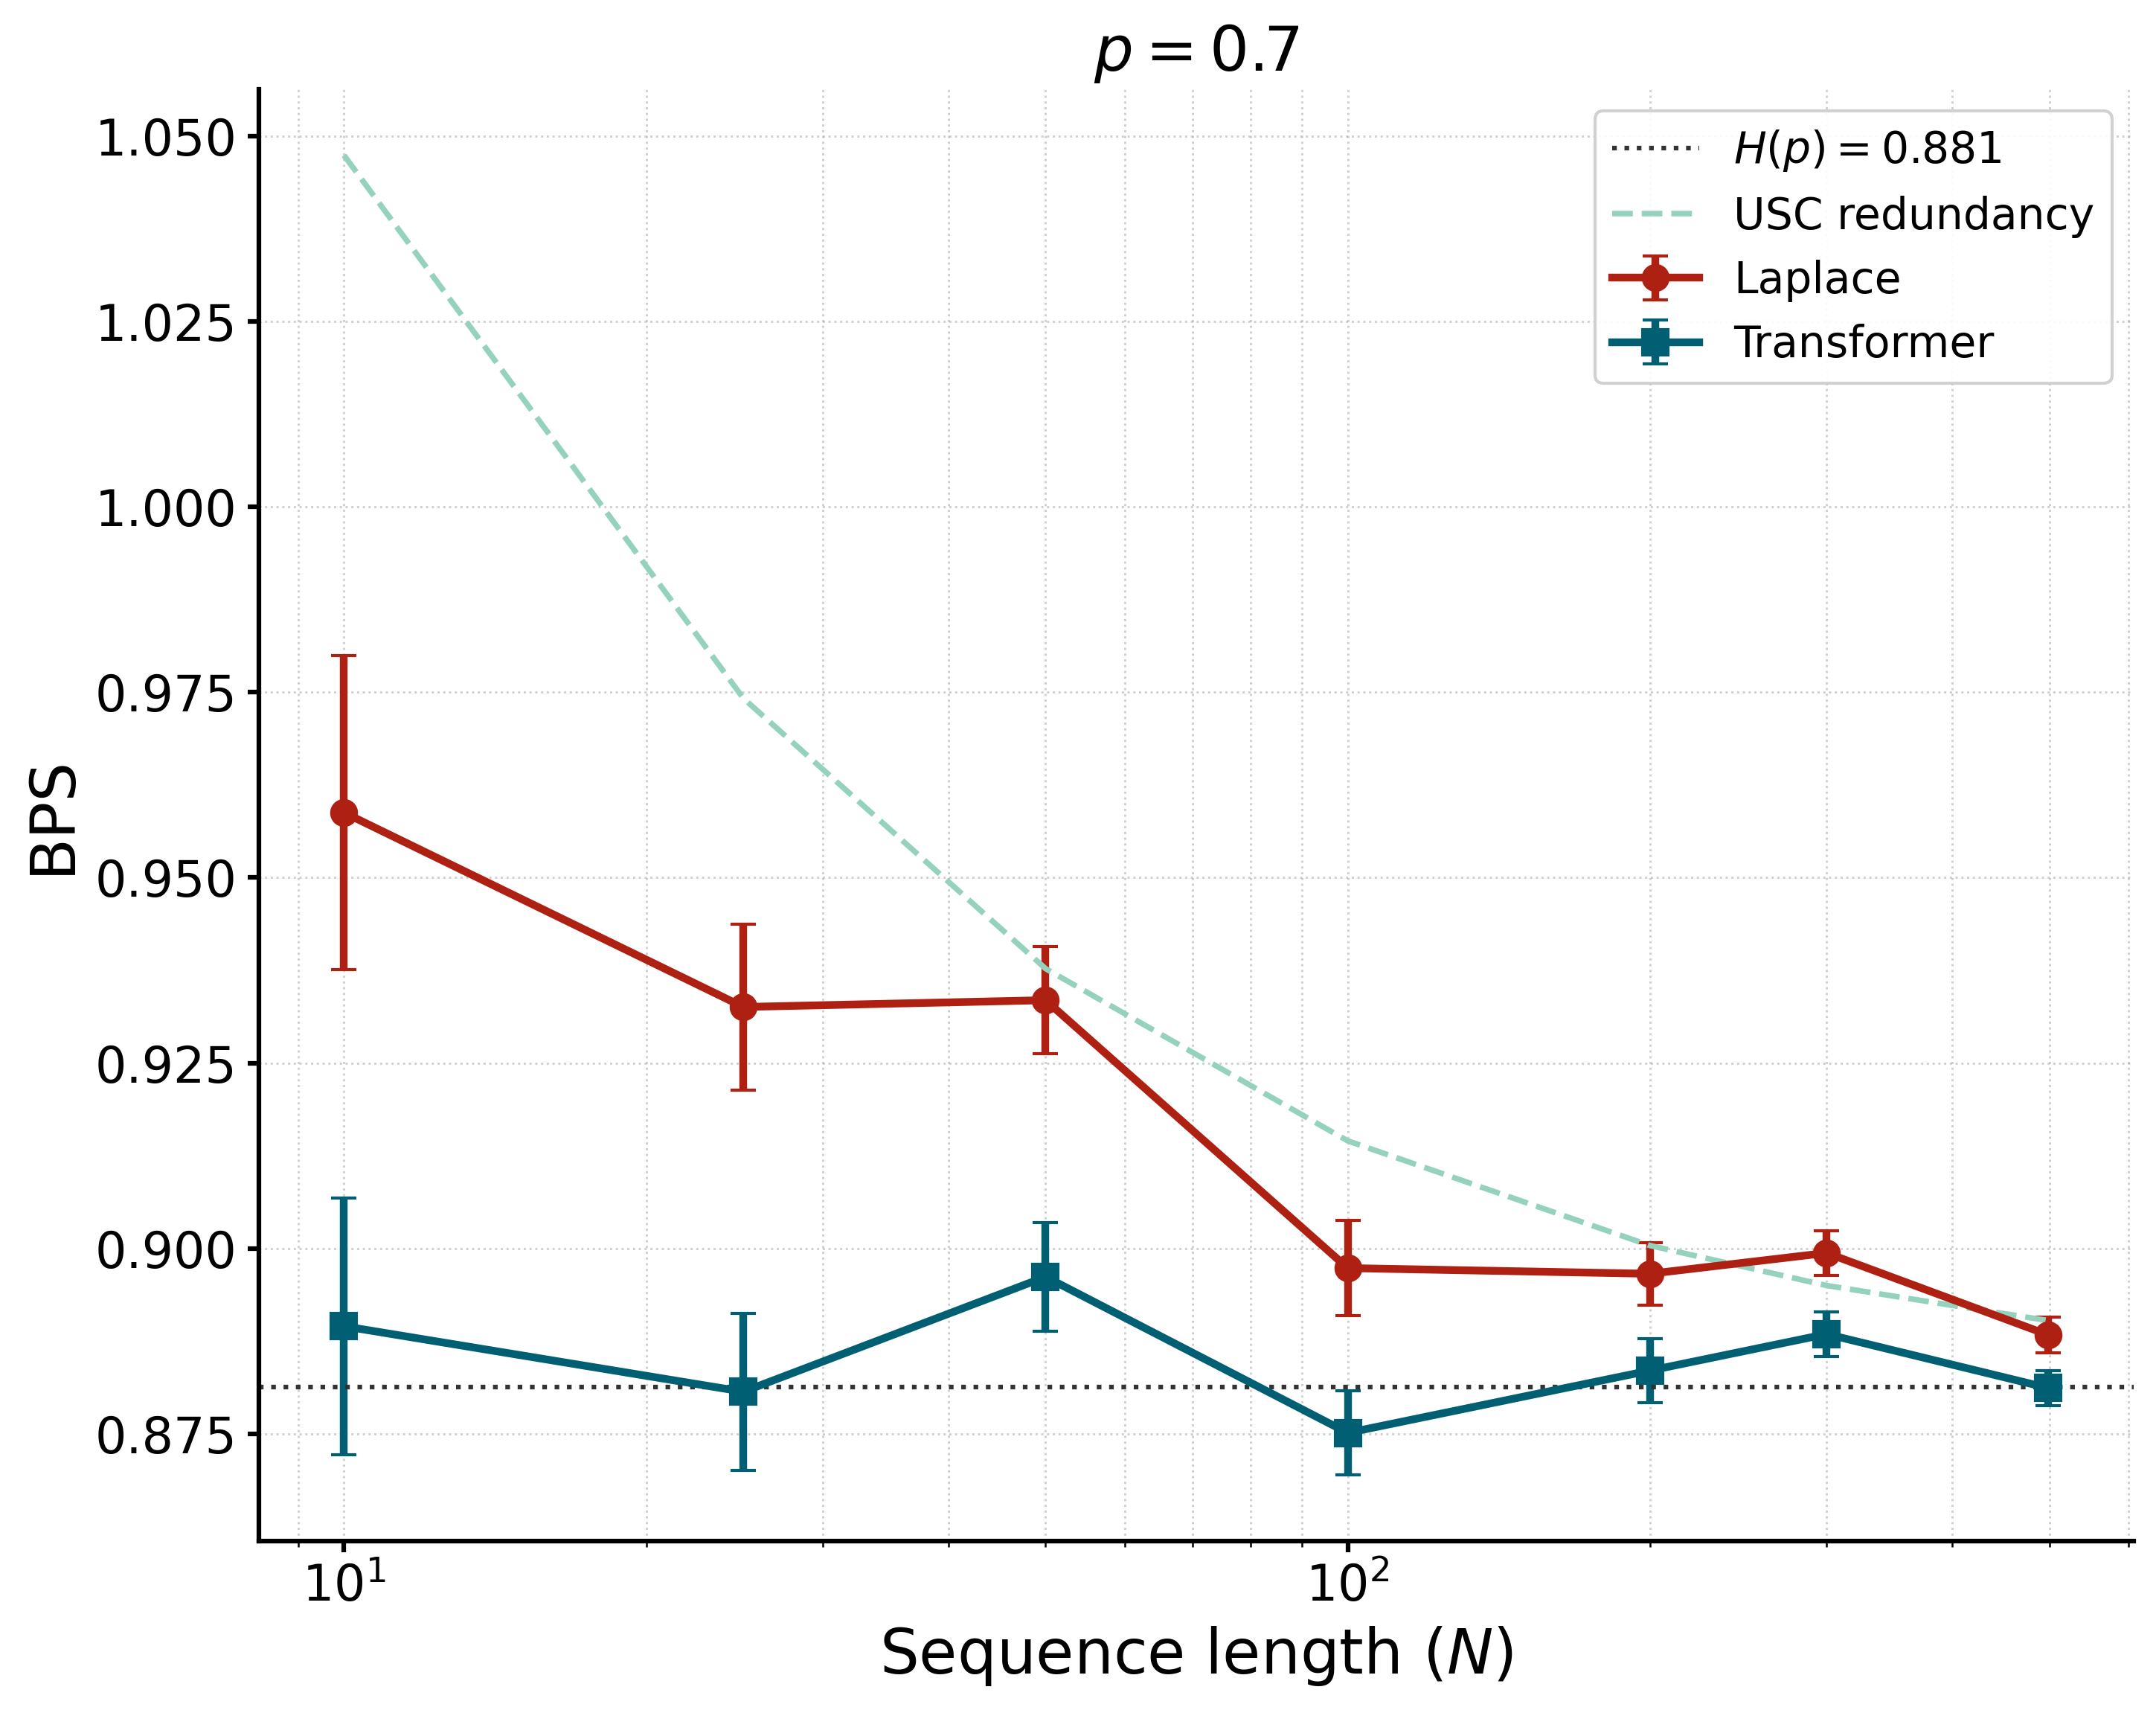
\includegraphics[width=\linewidth]{figures/iid_bps_p07.png}
    \end{center}
    {\small \textbf{Figure 2b.} Specialized model ($p{=}0.7$). Same pattern the
    transformer's baked-in prior gives it a head start Laplace cannot match at small $N$.}
  \end{column}
\end{columns}

\medskip
\vspace{1.5ex}
The advantage is largest at small $N$, persisting 
throughout Laplace as it asymptotically approaches the entropy floor. Meanwhile, the transformer is
already there from the first token.

\vspace{1.5ex}
\bigskip
%----- FSM + Redundancy side by side ------------------
\begin{columns}[t]
  \begin{column}{0.5\linewidth}
    \textbf{FSM sources: transformer dominates.}
    The 4-state FSM with emission probabilities $[0.1, 0.35, 0.65, 0.9]$ and 
    Dirichlet-sampled transition matrices ($\alpha = 1.0$) represents a single 
    configuration of a much larger experimental space. Results shown here are for one FSM configuration; concentration parameter $\alpha$ and state count are both axes for future exploration.
    \begin{center}
      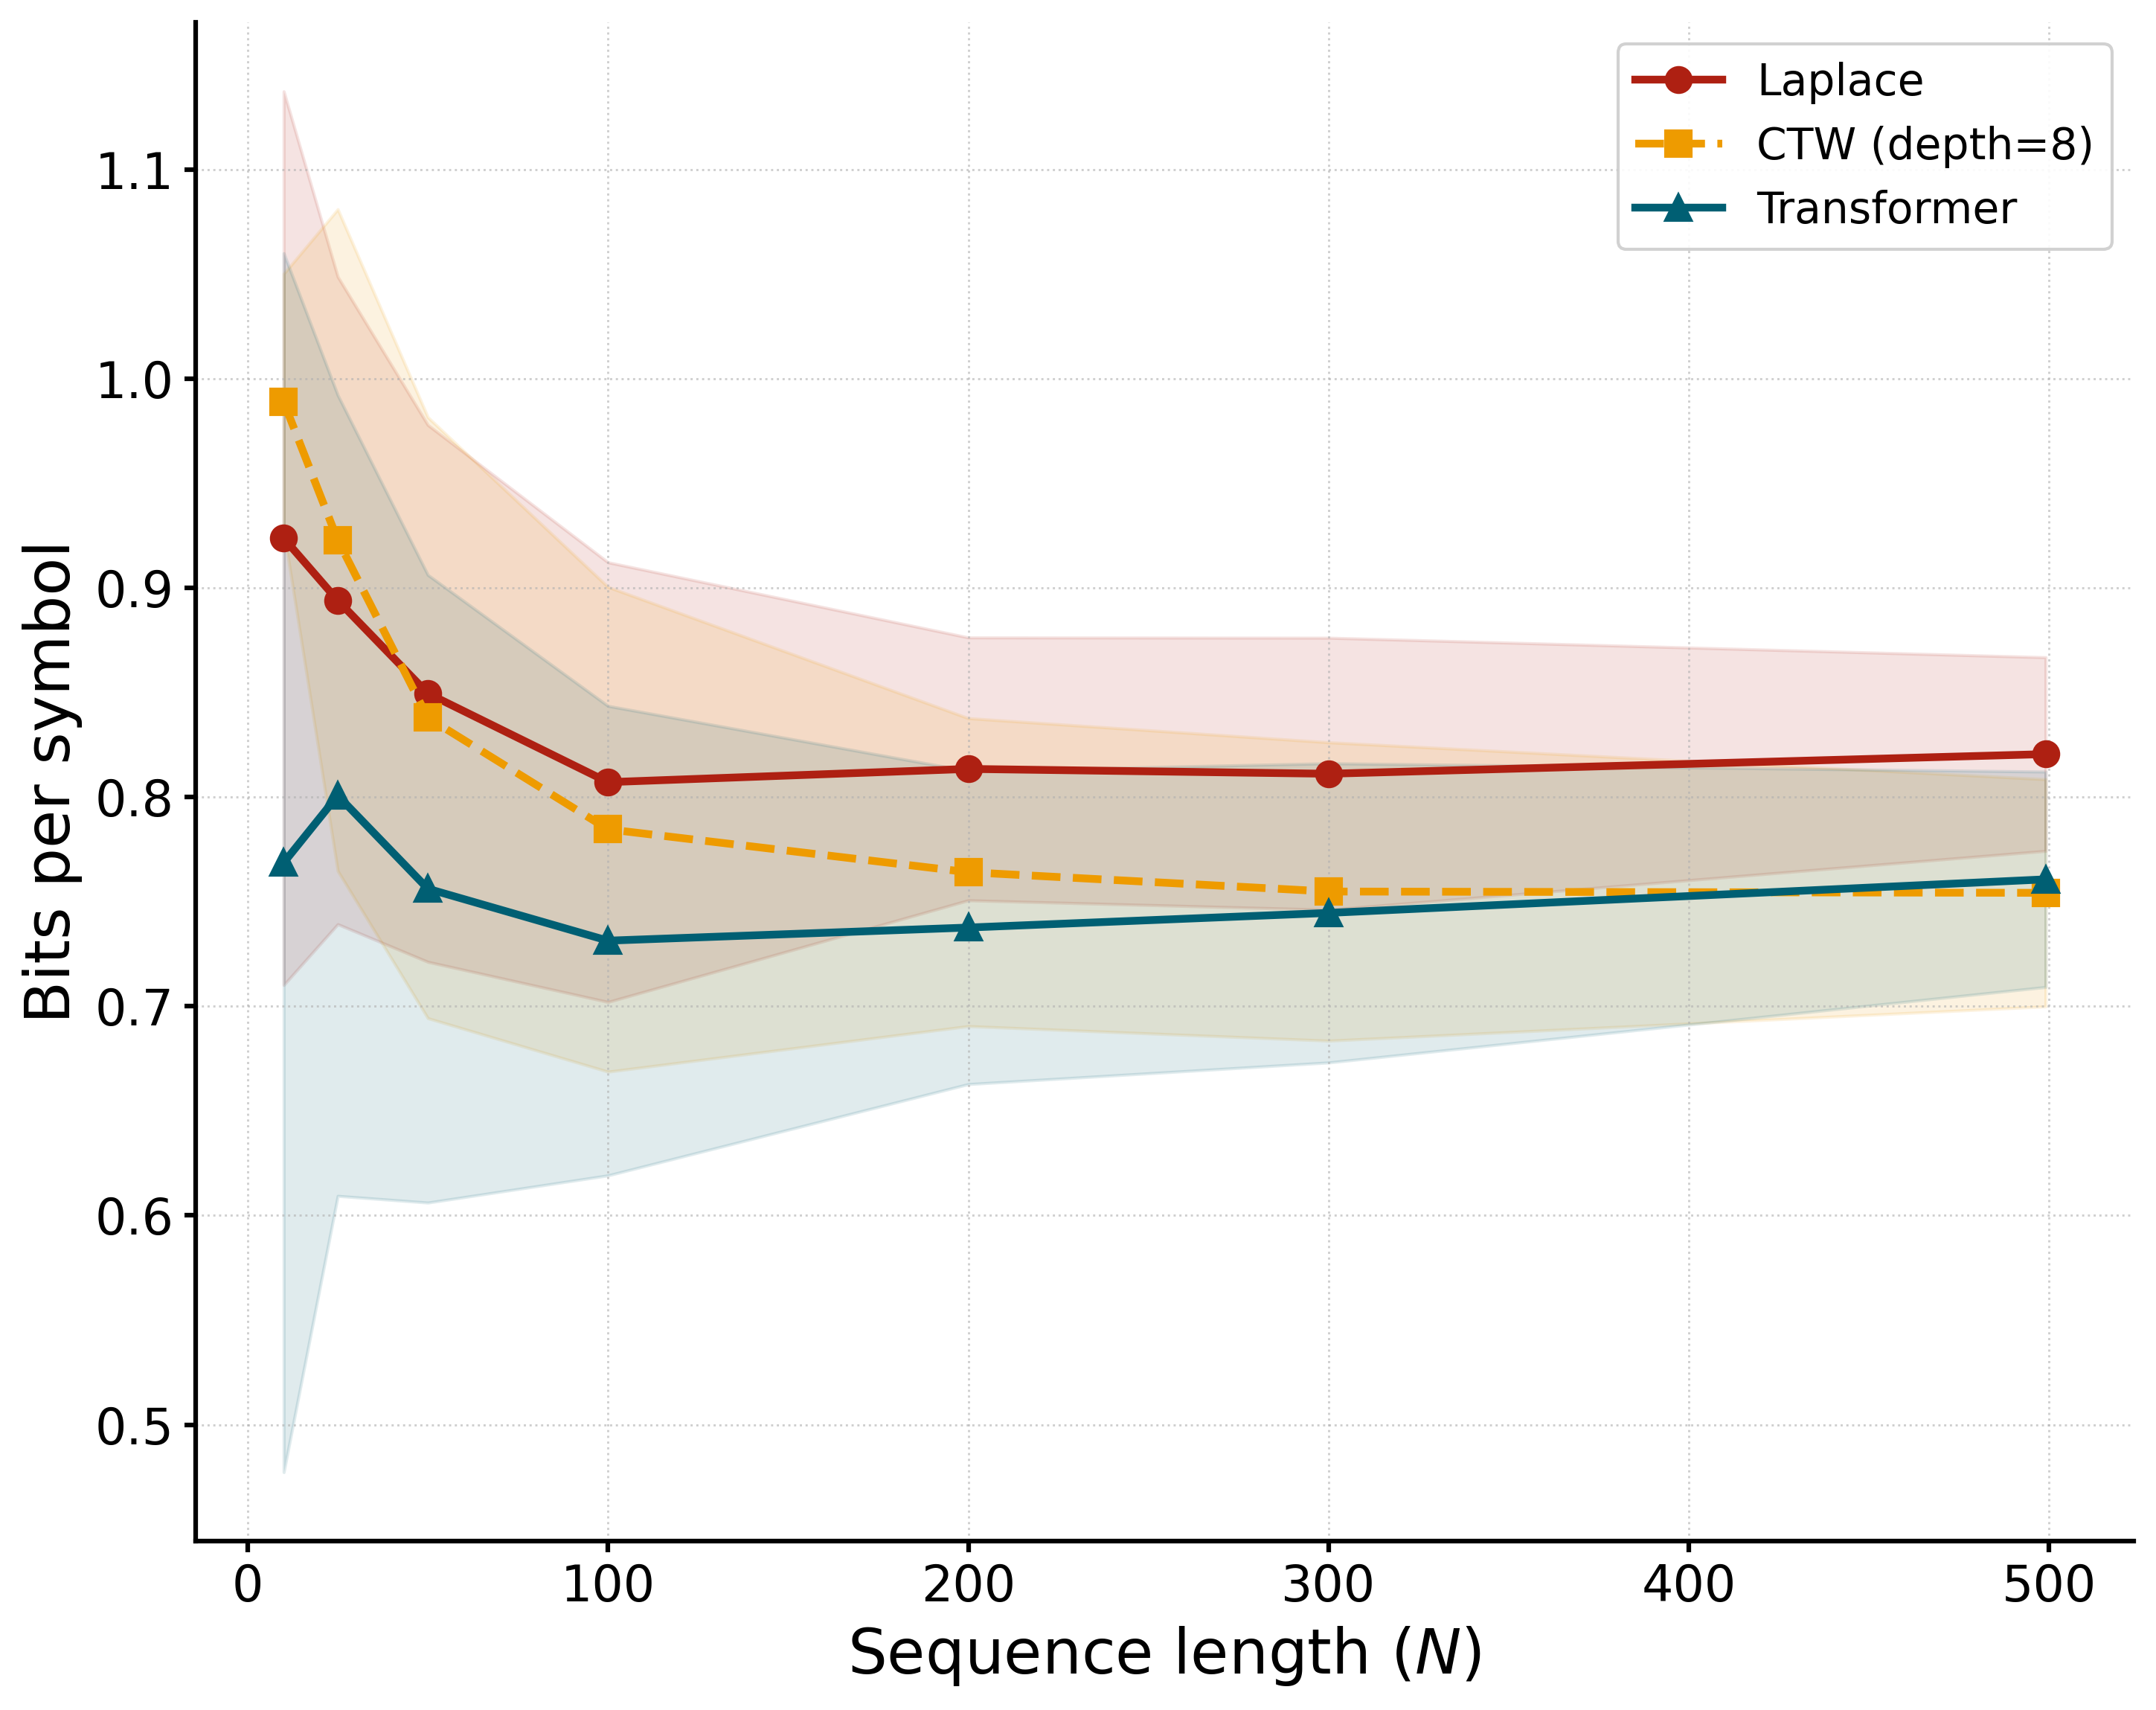
\includegraphics[width=\linewidth]{figures/fsm_benchmark.png}
    \end{center}
    {\small \textbf{Figure 3.} BPS vs.\ $N$ for the 4-state FSM.
    Transformer ({\color{tealblue}$\blacktriangle$}) beats both Laplace
    ({\color{alertred}$\bullet$}) and CTW ({\color[RGB]{238,155,0}$\blacksquare$})
    at every $N$. CTW outputs $0.97$ BPS at $N{=}10$ (nearly incompressible)
    due to depth-8 warmup cost. Shaded bands: $\pm 1$ SD.}
  \end{column}
  \begin{column}{0.5\linewidth}
    \textbf{Learning rate confirms theory.}
    Redundancy follows $R^{+}_\ell(m) = \frac{1}{2m\ln 2} + o(1/m)$, predicting 
    a $1/m$ decay with growing training samples. The transformer crosses the Laplace 
    baseline near $m \approx 80$
    \begin{center}
      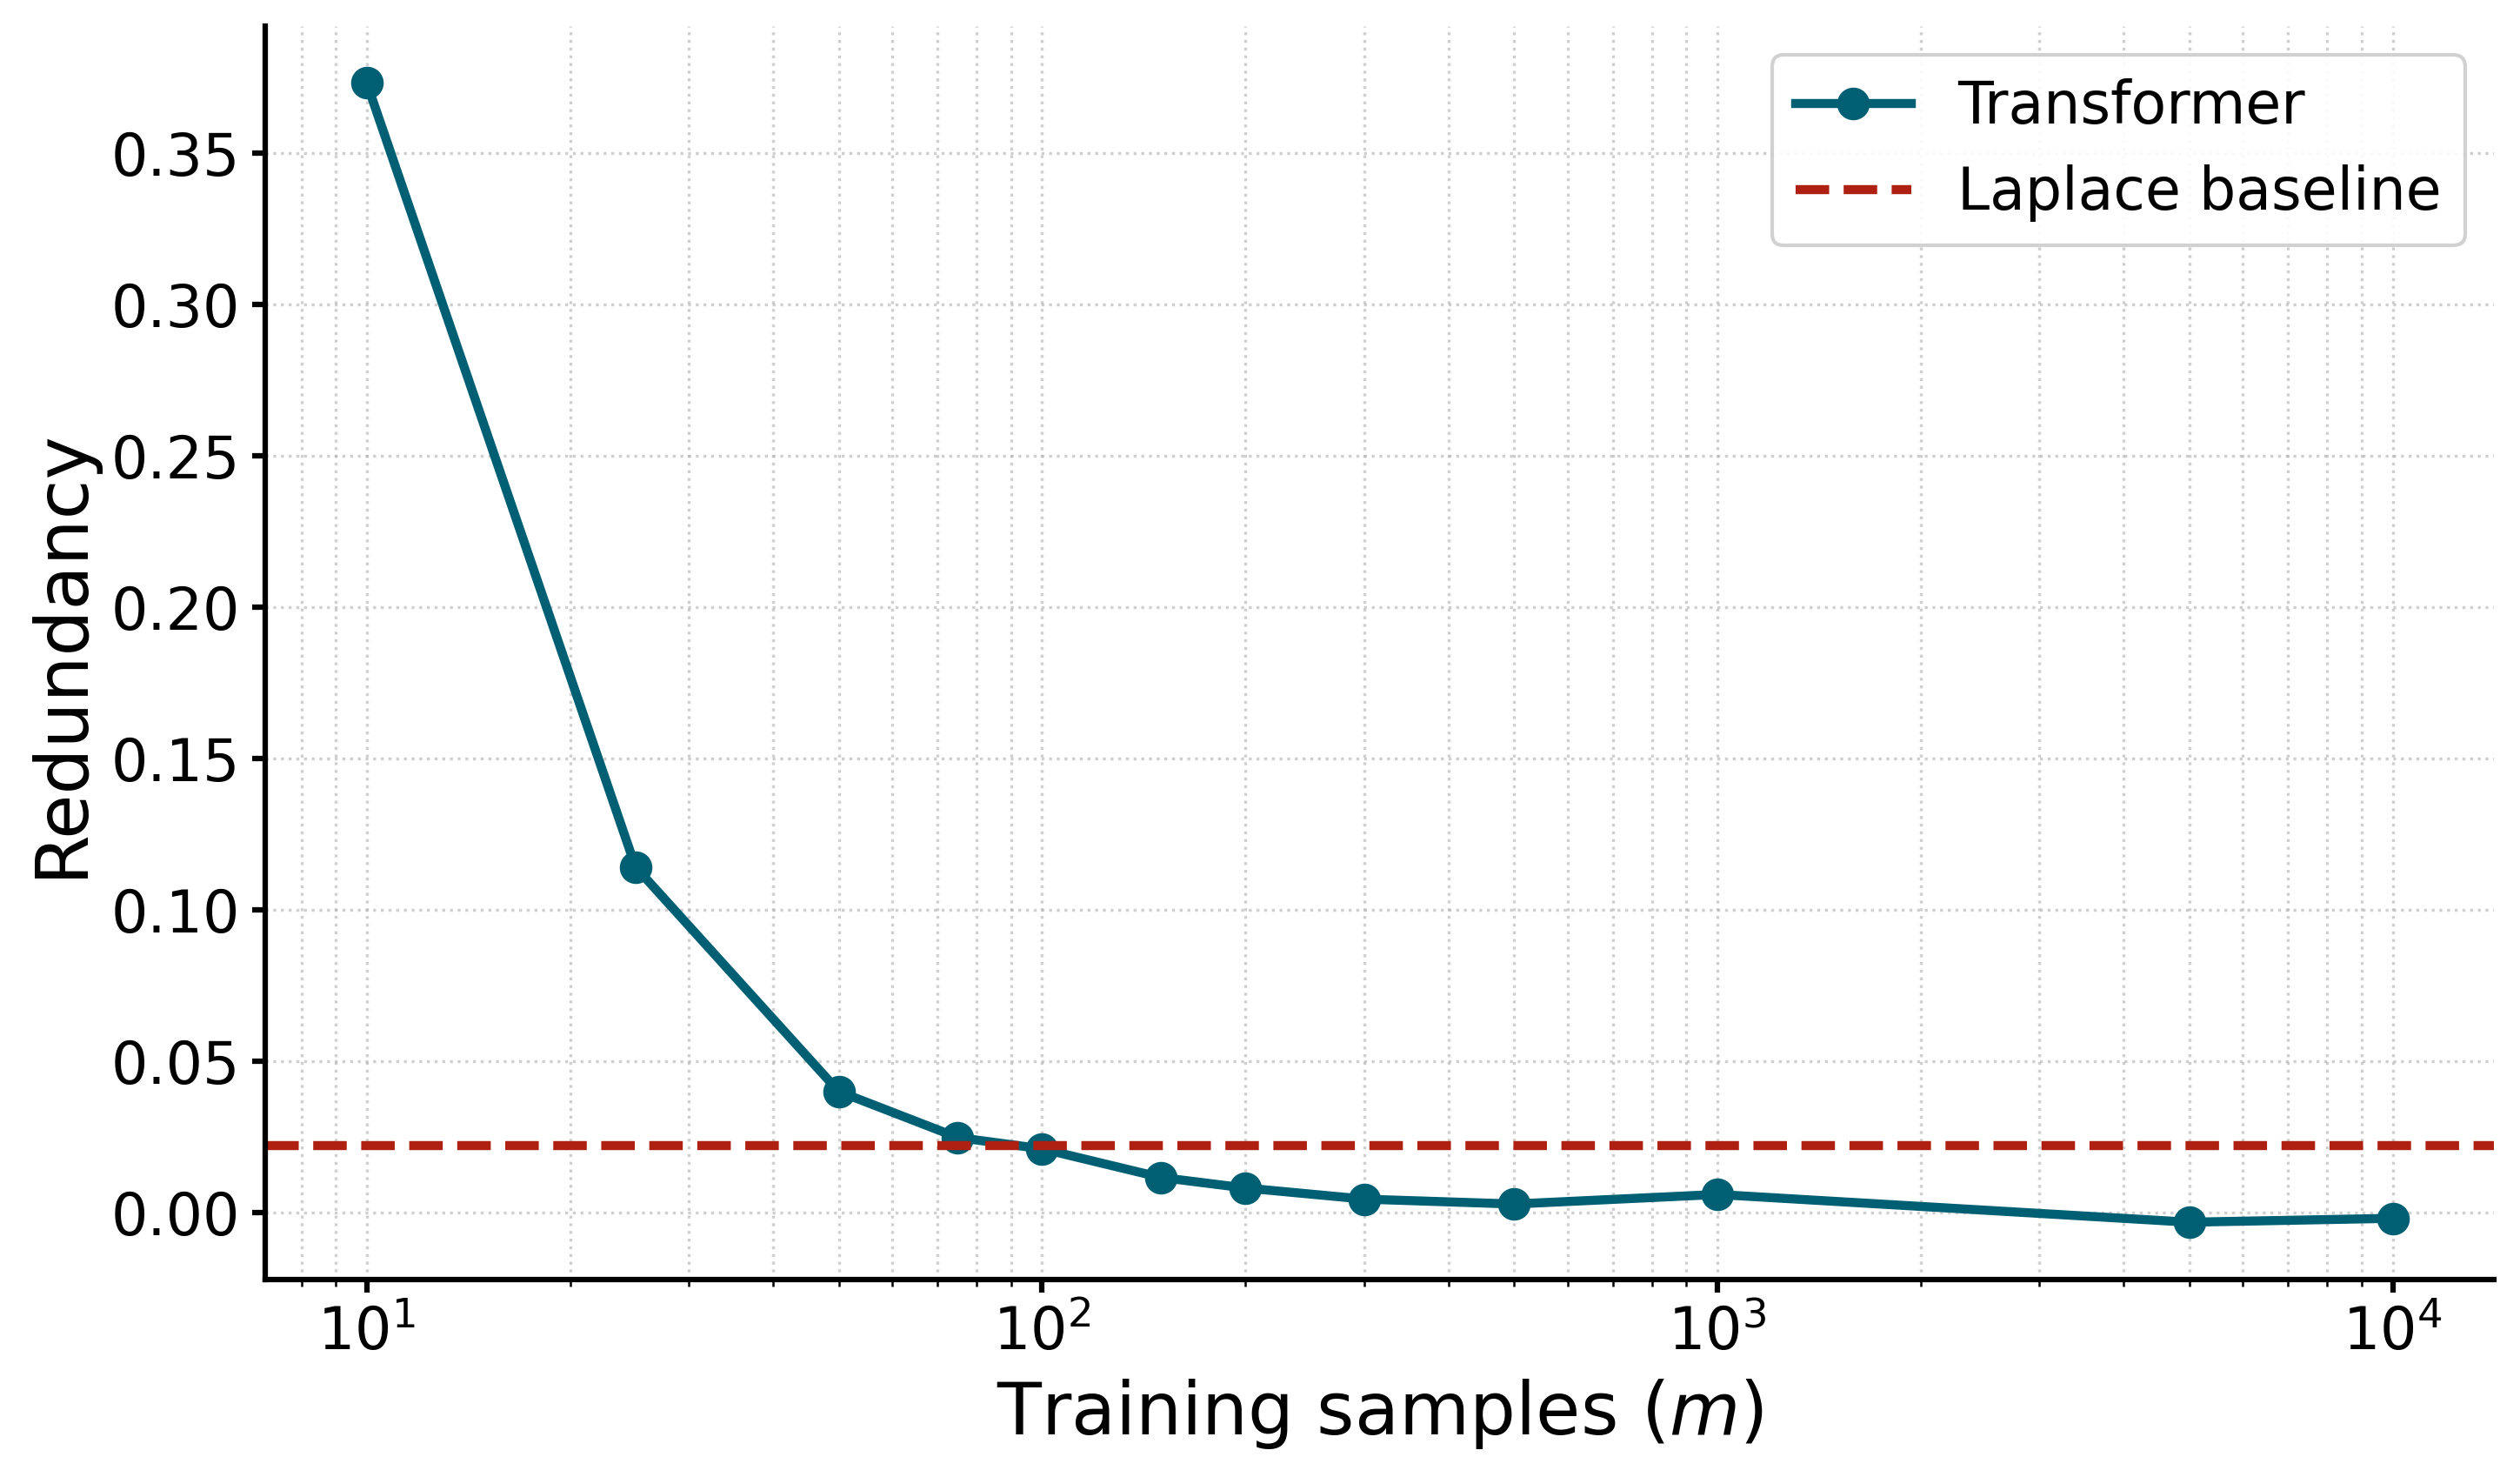
\includegraphics[width=\linewidth]{figures/redundancy_vs_training.png}
    \end{center}
    {\small \textbf{Figure 4.} Redundancy vs.\ training sequences $m$
    (IID, $p{=}0.3$, $N{=}499$) at around $10^2$, training samples, the transformer begins to demonstrate compression gains over Laplace estimation}
  \end{column}
\end{columns}
\end{block}

\begin{block}{Acknowledgements}

\small
We thank \textbf{Prof.\ Anders H\o{}st-Madsen} (UH Manoa ECE) for advising
this project and for the theoretical framework in \emph{Bounds for Learning Lossless Source
Coding} (arXiv:2009.08562, 2020) that motivates this empirical study.
Department of Electrical \& Computer Engineering, University of Hawai\textquoteleft{}i
at M\=anoa, Spring 2026.

\end{block}

\end{column} % end RIGHT COLUMN

\begin{column}{\sepwid}\end{column}

\end{columns}
\end{frame}
\end{document}